\documentclass{article}
 
\usepackage[final, nonatbib]{nips_2017}

\usepackage[utf8]{inputenc} % allow utf-8 input
\usepackage[T1]{fontenc}    % use 8-bit T1 fonts
\usepackage{hyperref}       % hyperlinks
\usepackage{url}            % simple URL typesetting
\usepackage{booktabs}       % professional-quality tables
\usepackage{amsfonts}       % blackboard math symbols
\usepackage{nicefrac}       % compact symbols for 1/2, etc.
\usepackage{microtype}      % microtypography
\usepackage{bookmark}
\usepackage{graphicx}
\usepackage{svg}

\graphicspath{{images/}}
\svgpath{{images/}}

\title{Batch Normalization in Neural Networks Applied To Document Analysis}

\author{
  Andrew D.~Stelter \\
  Department of Computer Science\\
  South Dakota School of Mines and Technology\\
  Rapid City, SD, 57701 \\
  \texttt{andrew.stelter@mines.sdsmt.edu} \\
}

\begin{document}
% \nipsfinalcopy is no longer used

\maketitle

\begin{abstract}
  The abstract must be limited to
  one paragraph.
\end{abstract}

\section{Introduction}

In the early 2000s, a Neural Nets were shown to be one of the best tools available for
document analysis and handwriting recognition. 
\cite{tay2001offline} \cite{sinha1999improved}
In their 2003 paper, Simard 
\cite{simard2003best} 
outlined a general-purpose neural net architecture that
is adequate for simple document analysis.

In their work, Simard achieved a 4\% error rate using a simple convolutional neural net to recognized digits from the MNIST 
\cite{mnist}
data set. Since the publishing of that paper, new general-purpose techniques have been developed which can be used to expand that architecture. In this paper, we compare that neural net's performance to the performance of one using one of those new techniques.

The technique in question is batch normalization as presented in 2015 by Sergey Ioffe and Christian Szegedy. 
\cite{ioffe2015batch}
Batch normalization can be used to accelerate the learning of neural nets by normalizing each batch of training data after each layer of the network. Doing this allows the gradients at each step to be independent of the data and gradients in other steps; this in turn allows the neurons of the neural net to learn at different rates.

We found...

\section{Methods}
In the original paper by Simard, it is indicated that they developed the neural network from scratch. We made the decision to use one of the many neural network frameworks which has been put together since that paper. The framework which was chosen is Torch. 
\cite{torch}

Using Torch allowed rapid development of a neural network to process the MNIST database. In fact, the Torch project provides a neural net to do this as one of its example projects. While this example proved invaluable while learning how to use Torch, it did not follow the architecture laid out by Simard, so it was ultimately only useful for seeing how a Torch neural net program might be structured.

\subsection{Expanding the Dataset}
In their original paper, Simard outlines a number of methods used to expand the training dataset. They used both affine transformations and elastic deformations to created noisy and warped versions of the original images. The Torch Images library provides functionality for part of this process, thus we did not need to recreate the entire algorithm form applying affine transforms and elastic deformations to an image. We tested the neural net by producing four sets of training data:
\begin{itemize}
  \item The original MNIST dataset
  \item The original MNIST dataset and some transformed versions of each image
  \item The original MNIST dataset and some deformed versions of each image
  \item The original MNIST dataset and both transformed and deformed versions of each image
\end{itemize}

\subsubsection{Transforming the Images}
Simard does not outline the specific rules used to generate their affine transformations. We picked a number of rules and used them to generate random 2x2 transformation matrices which could then be applied to the images. Each transform consisted of the following elements:
\begin{itemize}
  \item A random rotation in the range $\pm\frac{\pi}{16}$ radians
  \item A random shearing in both the x and y dimensions of $\pm 0.125$
  \item A random scaling in both the x and y dimensions of $\pm 0.25$
\end{itemize}

These are the ranges which were found to generate as much variance in the images as possible without changing them to the point of being unrecognizable. Some examples transformations can be seen in Figure~\ref{fig:transforms}.

\begin{figure}
  \centering
  \includegraphics[width=0.15\textwidth]{original.png}
  \includegraphics[width=0.15\textwidth]{transform1.png}\\
  \includegraphics[width=0.15\textwidth]{transform2.png}
  \includegraphics[width=0.15\textwidth]{transform3.png}
  \label{fig:transforms}
  \caption{One of the original images (top left) and some examples of its affine tranformations}
\end{figure}

\subsubsection{Warping the Images}

As stated above, the Torch Images library provides much of the functionality needed to recreate the elastic deformations described by Simard. Their description of the process described convolving two delta fields $\delta x$ and $\delta y$ with a gaussian of some standard deviation $\sigma$. The resulting displacement field could be scaled by some $\alpha$ and then applied to the original image to warp it.

Using the Torch Image library simplified this process greatly, and we were able to quickly start creating deformed data sets to test with. At the recommendation of Simard, we used $\sigma=4$ and $\alpha=34$; however, it is unknown whether or not the displacement fields produced through Torch were analogous to the ones produced by their algorithm. Some example vector fields and their resulting deformations can be seen in Figure~\ref{fig:deforms}.

\begin{figure}
  \centering
  \includegraphics[width=0.15\textwidth]{original.png}
  \includesvg[width=0.2\textwidth]{deform1.svg}
  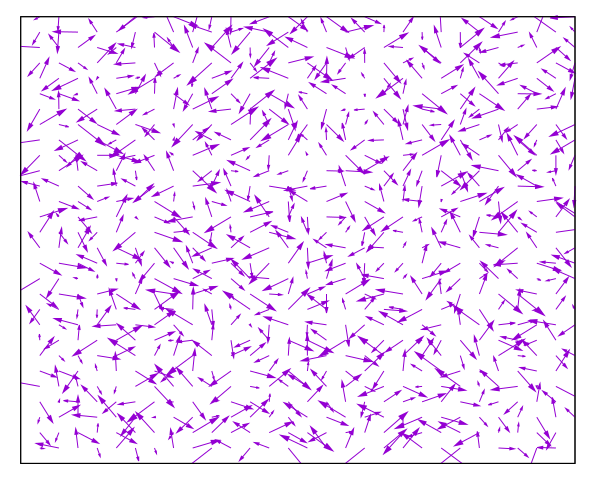
\includegraphics[width=0.15\textwidth]{deform1.png}\\
  \includesvg[width=0.2\textwidth]{deform2.svg}
  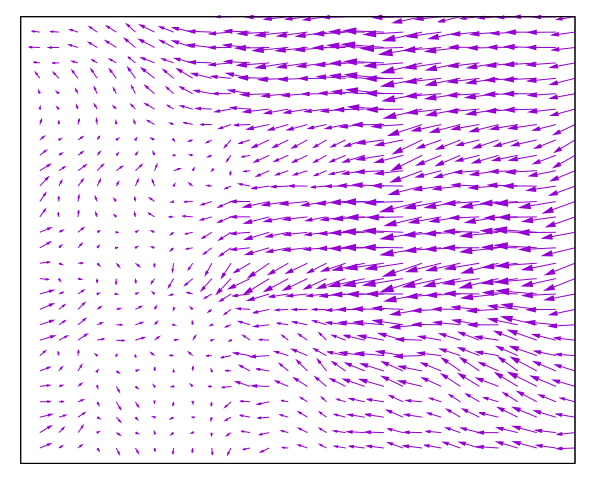
\includegraphics[width=0.15\textwidth]{deform2.png}
  \includesvg[width=0.2\textwidth]{deform3.svg}
  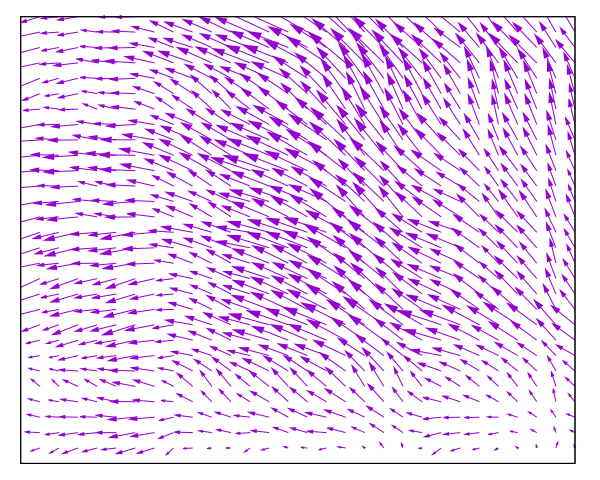
\includegraphics[width=0.15\textwidth]{deform3.png}
  \label{fig:deforms}
  \caption{One of the original images (top left) and vector fields with their resulting deformations. In order: $\sigma=0.001$, $\sigma=4$, and $\sigma=30$}
\end{figure}

\subsection{Network Architecture}
The network architecture outlined by Simard can be described succinctly as a feature extractor followed by a universal classifier. The feature extraction portion consisted of two spatial convolution layers, each having a kernel of size 5. This reduced the input image from 29x29 pixels to 5x5 pixels. The first layer of convolution output 5 planes size 13x13, and the second layer produced 50 planes. The universal classifier is described as two fully connected layers of neurons, sizes 100 and 10 respectively, with the layer of 10 being the output layer. The final error calculation was done using both Mean-Squared-Error and Cross-Entropy calculations.

Building the same neural net in Torch was fairly simple; however, a couple of minor changes were made as a result. The biggest difference was the connection between the feature extractor and the classifier. The feature extraction ended with a total of 1250 pixels in all of its planes combined. In order to feed this data into the universal classifier, an extra fully connected layer of the same size had to be added between the extractor and the classifier. The second change was that we tested only with a cross-entropy error calculation; mean-squared-error was not tested in this project. Finally, Simard does not note the transfer function used between the layers of his net. At the recommendation of the Torch quickstart tutorial \cite{torchTutorial} for identifying images in the CIFAR data set \cite{krizhevsky2009learning}, we used a ReLU transfer function between all layers of the neural net.

\subsection{Batch Normalization}
The main goal of this project was to determine how batch normalization as described by Ioffe and Szegedy would affect the network laid out by Simard. To this end, we made use of the Torch SpatialBatchNormalization and BatchNormalization layers after the convolution layers and linear layers, respectively. These layers were allowed to learn their $\beta$ and $\gamma$ parameters during training; the values were not taken from the dataset or provided as constants.

The power of batch normalization comes from training the neural net on small sets of the full training set known as minibatches. For each epoch trained, a random permutation of the full training set was generated. Then minibatches were made by taking sequential groups of $n$ items. Each minibatch was trained during that epoch as if it were a full training set. Picking minibatch sizes can be difficult and depends on the application of the neural net, so we tested our net using multiples of 100 up to 1000 which evenly divided the full training set size to see what yielded the best result.


\section{Results}

\section{Analysis}

\subsection{Tables}

The table
number and title always appear before the table.  See
Table~\ref{sample-table}.

Place one line space before the table title, one line space after the
table title, and one line space after the table. The table title must
be lower case (except for first word and proper nouns); tables are
numbered consecutively.

Note that publication-quality tables \emph{do not contain vertical
  rules.} We strongly suggest the use of the \verb+booktabs+ package,
which allows for typesetting high-quality, professional tables:
\begin{center}
  \url{https://www.ctan.org/pkg/booktabs}
\end{center}
This package was used to typeset Table~\ref{sample-table}.

\begin{table}[t]
  \caption{Sample table title}
  \centering
  \begin{tabular}{lll}
    \toprule
    \multicolumn{2}{c}{Part}                   \\
    \cmidrule{1-2}
    Name     & Description     & Size ($\mu$m) \\
    \midrule
    Dendrite & Input terminal  & $\sim$100     \\
    Axon     & Output terminal & $\sim$10      \\
    Soma     & Cell body       & up to $10^6$  \\
    \bottomrule
  \end{tabular}
  \label{sample-table}
\end{table}

\section{References}
\bibliographystyle{IEEEtran}
\bibliography{sources}

\end{document}
